\documentclass[pdftex,12pt,a4paper]{article}
\usepackage[pdftex]{graphicx}
\usepackage{fancyhdr}
\usepackage{geometry}
\usepackage{draftcopy}
\usepackage{float}
\usepackage{amsmath}
\usepackage{algorithm2e}
\usepackage{color, colortbl}
\definecolor{Gray}{gray}{0.9}
\renewcommand{\thesection}{\arabic{section}.}
\renewcommand{\thesubsection}{\arabic{section}.\arabic{subsection} }
\renewcommand{\headrulewidth}{0pt}
\renewcommand{\footrulewidth}{0.5pt}
\pagestyle{fancy}
\fancyhead{}
\fancyfoot[LE,LO]{\footnotesize{
SE344, Chemistry and Our Environment
}
}

\title{\vspace{-15pt}Alternative Technologies for Chemical Containment\\ SE344: Chemistry and Our Environment}
\author{Ankesh Kumar Singh (Y9090)}
\date{22nd March, 2013}
\begin{document}
\maketitle
\begin{tabular}{p{370pt}}
\textbf{Keywords: }BP oil spill, CI agent, containment of chemicals
\end{tabular}
\vspace{10pt}\\
\hrule
\vspace{10pt}
At a time of a crisis, a number of ideas come up. It is not always possible to go through each of them, but many of them may be a good solution to the problem. The Deepwater Horizon Oil Spill (BP Oil Spill) was one of the worst oil disasters in history. In the BP Oil Spill, more than 200 million gallons of crude oil was pumped into the Gulf of Mexico for a total of 87 days, making it the biggest oil spill in U.S. history. 16,000 total miles of coastline have been affected, including the coasts of Texas, Louisiana, Mississippi, Alabama, and Florida.

Even though the gushing well was capped in July 2010, oil is still washing up on shores, which might cause long-term damages to people living in the area. The initial oil rig explosion killed 11 people and injured 17 others. One method of treating the oil spill is "in-situ burning" or burning oil in a contained area on the surface of the water, which has negative effects on the environment. Another method was by the use of trawlers, where water is pumped into the ship, oil is separated out from it and then water is releases back to the sea. This process is expensive and requires high man power. BP is responsible for close to \$40 billion in fines, cleanup costs, and settlements as a result of the oil spill in 2010, with an additional \$16 billion due to the Clean Water Act.

An innovative solution to cleanup of spill was proposed by C.I.Agent Solutions a Louisville, Kentucky based startup. Oil can be contained by using solidifiers that consist of hydrophobic dry granular material made up of polymers. It physically absorbs oil to form a cohesive solidified mass that floats on water surface. Oil may be later recovered from this solid. These were experimented in EPA approved tanks and pond sections. However, this presentation was rejected by British Petroleum as the polymer was expensive. Further, archived reports of all the proposed solutions were not shared publicly. So an alternative technology is never brought to general awareness.
\begin{center}
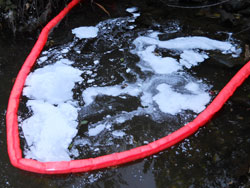
\includegraphics{cia.jpg}
\end{center}

This brings us to a proposition regarding alternative technologies as to what can be done differently for these to be implemented. People involved in such technologies must be engaged at Congress level and as a part of National Response teams. Entrepreneurs and industry leaders bring in a lot of expertise in this regard.

An industrial spill can never be prevented. Containment of a disaster is carried out only after personnel have been moved to safety.
\end{document}